\documentclass[12pt]{article}

\usepackage{stoversymb,graphicx,soul, changepage}
\usepackage[letterpaper, margin=0.5in, top=0.75in, bottom=1in]{geometry}

%\everymath{\displaystyle}

\usepackage{multicol}
\usepackage[many]{tcolorbox}
\usepackage{tikz}

\title{\vspace{-0.75in}\LARGE{Fundamental Ideas in Vector Calculus\\(and how to keep them separate)}\vspace{-1in}}
\date{}

\usepackage[inline]{enumitem}
\setlist[enumerate,1]{leftmargin=0.625in, rightmargin=0.5in, label=(\alph*),itemsep=2.25mm,topsep=1.5mm}
\setlist[enumerate,2]{leftmargin=0.25in}
\setlist[itemize]{topsep=-1.5mm}

\renewcommand{\Q}{\vspace{4.5mm}\noindent\textbf{Question}: }
\newcommand{\Ans}{\ul{Answer}: }
\newcommand{\Short}{\ul{Short Answer}: }
\newcommand{\Long}{\vspace{3mm}\ul{Longer Answer}: }
\newcommand{\shortlim}{\lim_{n\to\infty}}
\newcommand{\sectitle}[1]{\vspace{7.5mm}\noindent\textbf{\Large{#1}}\\[3mm]}
\newcommand{\subsectitle}[2]{\vspace{3mm}\noindent\ul{#1}:\\[3mm]\indent{#2}}
\newcommand{\subsecnoindent}[2]{\vspace{3mm}\noindent\ul{#1}:\\[3mm]{#2}}
\newcommand{\comps}[1]{\langle #1_1,#1_2,#1_3\rangle}
\newcommand{\compslong}[3]{\langle #1, #2, #3\rangle}
\newcommand{\pic}[2]{\begin{center}\includegraphics[scale=#1]{#2}\end{center}}
\newcommand{\resultbox}[1]{\begin{center}
		\begin{tcolorbox}[
			enhanced,
			colback=white,
			colframe=black,
			boxrule=0.5pt,
			arc=0pt,
			top=3mm,
			bottom=3mm, 
			width=7in%,
%			grow to left by=0.5in,
			]
			\centering
			#1
		\end{tcolorbox}
\end{center}}
\newcommand{\LH}{L'H\^{o}pital}

\graphicspath{ {./img/} }
\DeclareGraphicsExtensions{.pdf, .png}

\usepackage{caption}
\captionsetup{labelfont=bf, labelformat=simple, justification=centering, labelsep=newline, width=6.5in, textfont={small}}%, textfont={it, footnotesize}}
\captionsetup[figure]{aboveskip=8pt, belowskip=10pt}

\begin{document}
	\setlength\parskip{4.5mm}
	
	\maketitle
	
	\noindent First, a rundown of what kinds of questions will be on your final.
	
	\begin{adjustwidth}{0.25in}{0.25in}
		\noindent \textbf{The new stuff}\\[1.5mm]
		\noindent This will account for approximately 20\%--30\% of the points.
		\begin{itemize}[topsep=1.5mm,parsep=-4.5mm,itemsep=6mm]
			\item one (perhaps multi-part) question on the divergence theorem (\S 16.9);
			\item one (perhaps multi-part) question on Stokes' theorem (\S 16.8);
		\end{itemize}
	
		\noindent\textbf{Test 4 stuff}\\[1.5mm]
		This will account for 20\%--45\% of the points.
		\begin{itemize}[topsep=1.5mm,parsep=-4.5mm,itemsep=6mm]
			\item one question like number 3;
			\item $\geq 1$ line integral (with one requiring Green's theorem);
			\item $\geq 1$ surface integral/flux problem.
		\end{itemize}\vspace{-4.5mm}
		\noindent Note that these can be combined with the new stuff in obvious ways. For example, you may have to find a line integral using the old methods for part (a) of a question, and then find the same line integral in part (b) using Stokes' theorem.\\[-4.5mm]
	
		\noindent\textbf{The old stuff}\\[1.5mm]
		This will account for the remaining points, and not all of the listed concepts will be tested and/or tested equally.
		\begin{itemize}[topsep=1.5mm,parsep=-4.5mm,itemsep=6mm]
			\item using double and triple integrals (which may or may not include polar, cylindrical, or spherical coordinates) to find areas/volumes and volumes/hypervolumes, respectively (e.g. questions 2 and 4 on exam 3);
			\item directional derivatives/gradients (e.g. questions 3b, 3c, and 3d on exam 2);
			\item optimization of 2-variable functions (e.g. question 4 on exam 2);
			\item tangents/normals/curvature/etc. of vector-valued functions (e.g. question 3 on exam 1).
		\end{itemize}
	
		\noindent\textbf{Miscellany}\\[1.5mm]
		Here's some random info about the final not covered above.
		\begin{itemize}[topsep=1.5mm,parsep=-4.5mm,itemsep=6mm]
			\item there \textbf{won't be} any matching questions (e.g. question 4 on exam 1);
			\item there \textbf{may or may not be} true/false questions; if there are, it will \textbf{only} be about the Chapter 16 stuff;
			\item you \textbf{won't} have to know trig identities;
			\item there \textbf{will not} be a formula sheet.
%			 \textbf{definitely} have to know the Chapter 16 formulas + the formulas for $\vect{T}$, $\vect{N}$, $\vect{B}$, $\kappa$, etc., from exam 1; you \textbf{also} have to know how to change between coordinate systems (+ what the Jacobians are in various coordinate systems)
%			
%			you \textbf{may or may not} have to know the other ones.
		\end{itemize}
%	
%		\noindent The true/false questions will be about the new stuff only.
%		
%		For example, it's \textit{true} that if a two-dimensional vector field $\vect{F}=P\vect{i}+Q\vect{j}$ is conservative, then $\frac{\partial P}{\partial y} = \frac{\partial Q}{\partial x}$; it's \textit{not true} that $\frac{\partial P}{\partial y} = \frac{\partial Q}{\partial x}$ implies an arbitrary vector field is conservative, however (e.g. $\vect{G}=P\vect{i}+Q\vect{j}+R\vect{k}$ requires $\Curl\vect{G}=\vect{0}$ to be conservative, and as a bunch of you learned from question 3(a) on Test 4, these aren't equivalent).
	\end{adjustwidth}
	\setlength\parskip{3mm}
	\newpage

	Now, let's answer some questions some of you may be struggling with!
	
	\Q What is a vector field?
	
	\Short It's a function!
	
	\Long It's a function that takes in a 2- or 3-dimensional vector and outputs a vector of the same length. Because it's a function, you're able to do all the normal stuff with it: You can do arithmetic, you can compose things by plugging vector functions into it, and you can do calculus things. 
	
	\Q What is a line integral?
	
	\Ans It's the ``space curve'' equivalent of a ``regular integral'' from Calculus I and II.
	
	In those courses, your world is the $xy$-plane: You imagine the graph of a function $y=f(x)$ ``living over'' the $x$-axis and the ``regular integral'' represents the area bounded between the graph and the axis.

	In this course, your world is $\Reals^3$: You can imagine making the ``old $x$-axis'' curvy and putting it in space, calling this ``curvy axis'' $C$, then considering the part of the graph of a two-variable function $z=f(x,y)$ which lives over $C$. The area of that chunk of graph is \textbf{precisely} what we mean when we write $\oint_C f(x,y)\,ds$!
	
	\Q Right, okay...but what is that \textit{vertical curtain} thing you talked about so much?
	
	\Ans It's just a useful visualization of what the above-mentioned chunk of graph looks like!
	\begin{minipage}{0.45\linewidth}
		\vspace{-9mm}
		\begin{center}
			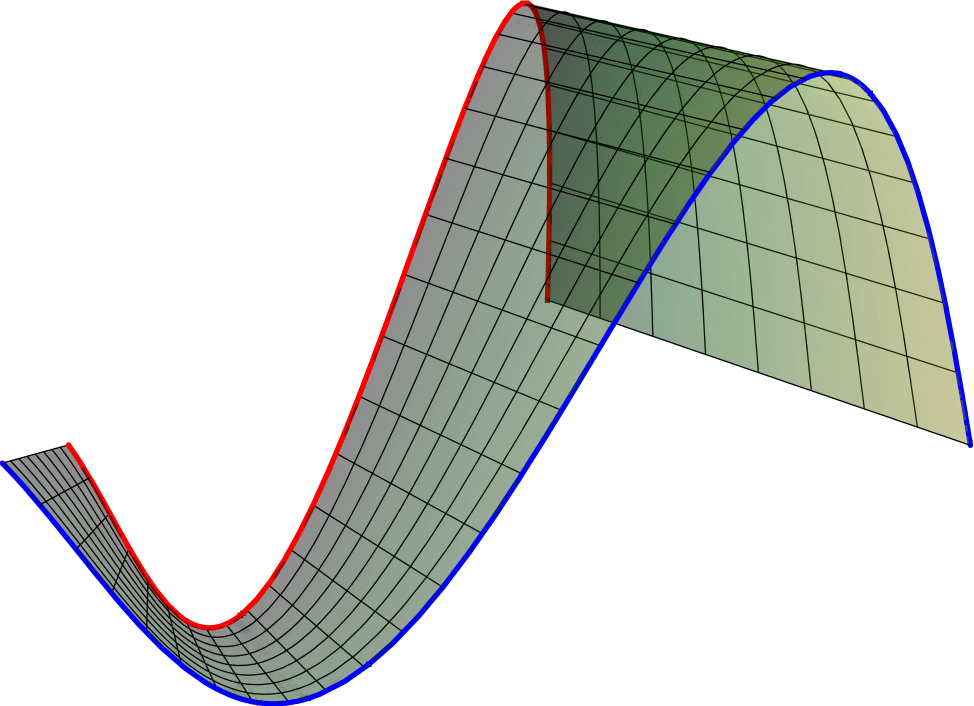
\includegraphics[scale=0.2]{calc2_smol}
		\end{center}
	\end{minipage}
	\begin{minipage}[b]{0.5\linewidth}
		\vspace{3mm}
		In this picture, the ``curvy axis'' $C$ is the red curve and the green ``curtain'' is the part of the graph of the two-var function $z=f(x,y)$ that lives above $C$ (with the blue ``top'' just there for visual precision).\par \vspace{3mm}
		
		With this visual, $\oint_C f(x,y)\,ds$ represents the area of that green curtain.
	\end{minipage}

	\Q Okay, so how do we compute line integrals?
	
	\Ans This answer kinda sorta depends on what the ingredients of the line integral look like.
	
	If you have a function $z=f(x,y)$, then your steps to compute $\oint_Cf(x,y)\,ds$ are as follows:
	\begin{itemize}[leftmargin=0.625in,rightmargin=0.5in,itemsep=0in]
		\item Find a parametrization of the form $x=x(t)$, $y=y(t)$, $a\leq t\leq b$ for $C$. For example: If $C$ is the upper half of the circle $x^2+y^2=1$, then you can use $x=\cos{t}$, $y=\sin{t}$, $0\leq t\leq \pi$.
		\item Plug $x=x(t)$ and $y=y(t)$ into $f(x,y)$ to get $f(x(t),y(t))$.
		\item Replace $ds$ with $\sqrt{[x'(t)]^2+[y'(t)]^2}\,dt$.
		\item Evaluate $\int_a^b f(x(t),y(t))\sqrt{[x'(t)]^2+[y'(t)]^2}\,dt$. Inside, this is multiplication of two scalars.
	\end{itemize}

	\Q How do we compute the line integral of a vector field?
	
	\Ans The process is very similar to the above.
	
	If you have a vector field $\vect{F}$, then the steps for computing $\oint_C\vect{F}\cdot d\vect{r}$ are as follows:
	\begin{itemize}[leftmargin=0.625in,rightmargin=0.5in,itemsep=0in]
		\setlength\parindent{0.25in}
		\item Find a vector function $\vect{r}(t)$, $a\leq t\leq b$, which parametrizes $C$. For example: If $C$ is the upper half of the circle $x^2+y^2=1$ like before, then you can use $\vect{r}(t)=\langle\cos{t},\sin{t}\rangle$, $0\leq t\leq \pi$.
		\item Plug $\vect{r}(t)$ into $\vect{F}$ to get $\vect{F}(\vect{r}(t))$. 
		
		If $\vect{r}$ and $\vect{F}$ are two-dimensional, this means you identify $\vect{r}(t)$ as $\vect{r}(t)=\langle x(t),y(t)\rangle$ and replace all $x$'s and $y$'s inside $\vect{F}$ with the $x(t)$ and $y(t)$ from $\vect{r}$; if they're three-dimensional, then $\vect{r}(t)=\langle x(t),y(t),z(t)\rangle$ and you replace the $x$'s, $y$'s, and $z$'s inside $\vect{F}$ with $x(t)$, $y(t)$, and $z(t)$.
		\item Replace $d\vect{r}$ with $\vect{r}'(t)dt$.
		\item Evaluate $\int_a^b \vect{F}(\vect{r}(t))\cdot\vect{r}'(t)\,dt$. Inside, this is dot product of two vectors (and thus a scalar).
	\end{itemize}

	\Q What does $\oint_C\vect{F}\cdot d\vect{r}$ represent \textit{physically}?
	
	\Ans That line integral represents the amount of work done by $\vect{F}$ on an object moving along $C$.

	\Q What is a conservative vector field?
	
	\Ans A vector field $\vect{F}$ (of any dimension) is \textit{conservative} if there exists a function $f$ for which $\vect{F}=\nabla f$. 
	
	Such vector fields are important, particularly in physics, because they tend to \textit{conserve} particular quantities in their respective systems.
	
	\Q How can I tell if $\vect{F}$ is conservative?
	
	\Ans There are lots of ways, but here are two good criteria (one for each of dimensions 2 and 3).
	
	Assuming $P$ and $Q$ have continuous first-order partial derivatives and that the 2D vector field $\vect{F}=P\vect{i}+Q\vect{j}$ is defined on an open, simply-connected domain in $\Reals^2$, then $\vect{F}$ is conservative if and only if 
	$$\frac{\partial P}{\partial y} = \frac{\partial Q}{\partial x}.$$
	
	Assuming $P$, $Q$, and $R$ have continuous partial derivatives and that the 3D vector field $\vect{F}=P\vect{i}+Q\vect{j}+R\vect{k}$ is defined on an open, simply-connected region in $\Reals^3$, then $\vect{F}$ is conservative if and only if $\Curl\vect{F}=\vect{0}$. This is true if and only if
	$$\frac{\partial R}{\partial y} = \frac{\partial Q}{\partial z}\quad\quad\quad\quad\frac{\partial P}{\partial z} = \frac{\partial R}{\partial x}\quad\quad\quad\quad\frac{\partial Q}{\partial x} = \frac{\partial P}{\partial y}$$
	all hold.
	
	On your test, it's a 99.9\% certainty that the vector fields you're given will be defined on all of $\Reals^2$ or $\Reals^3$, in which case the conclusions of these criteria may be used without checking the hypotheses.
	
	%		For example, it's \textit{true} that if a two-dimensional vector field $\vect{F}=P\vect{i}+Q\vect{j}$ is conservative, then $\frac{\partial P}{\partial y} = \frac{\partial Q}{\partial x}$; it's \textit{not true} that $\frac{\partial P}{\partial y} = \frac{\partial Q}{\partial x}$ implies an arbitrary vector field is conservative, however (e.g. $\vect{G}=P\vect{i}+Q\vect{j}+R\vect{k}$ requires $\Curl\vect{G}=\vect{0}$ to be conservative, and as a bunch of you learned from question 3(a) on Test 4, these aren't equivalent).
	
\end{document}